\documentclass[12pt]{article}
\usepackage{polski}
\usepackage[utf8]{inputenc}
\usepackage[OT4]{fontenc}
\usepackage{blindtext}
\usepackage[a4paper, total={6in, 9in}]{geometry}
\usepackage{hyperref}
\usepackage{graphicx}
\usepackage{listings}
\hypersetup{colorlinks=true,
linkcolor=,
urlcolor = blue}
\title{CMS}
\author{Damian Ćwikliński}

\begin{document}
\begin{titlepage}
    \begin{center}
        \vspace*{4cm}
            
        \Huge
        \textbf{System Zarządzania Stroną Siłowni}
            
        \vspace{0.5cm}
        \LARGE
        Systemy Zarządzania Treścią
            
        \vspace{1.5cm}
            
        \textbf{Damian Ćwikliński 145387}
            
        \vfill
            
        Politechnika Poznańska
            
        \vspace{0.8cm}
           
            
        prowadzący dr inż. Michał Apolinarski
            
    \end{center}
\end{titlepage}

\tableofcontents

\newpage
\section{Charakterystyka ogólna projektu}
Projekt zakłada stworzenia systemu zarządzania stroną internetową zawierającą informacje o siłowni i jej ofercie. 
\\

Aplikacja składająca się z części serwerowej oraz klienckiej ma pozwalać na edytowanie treści strony przez nieznającego się na programowaniu użytkownika. Użytkownik ma mieć możliwość zmiany zdjęć, informacji oraz banerów bez stosowania kodu.
\\

Poza zmianą treści głównej strony użytkownik powinien również mieć możliwość dodawania artykułów dotyczących wydarzeń organizowanych przez siłownię bądź też innych nowości związanych z placówką.
\\

Do stworzenia warstwy wizualnej inspiracja została zaczerpnięta ze strony \href{https://demo.templatemonster.com/demo/51682.html}{TemplateMonster}.

\newpage
\section{Wymagania}
\subsection{Funkcjonalne}
Wymagania z podziałem na role użytkowników:
\subsubsection{Redaktor}
\begin{itemize}
\item edycja, dodawanie, usuwanie artykułów i kategorii
\item edycja banerów strony (tekst i obraz)
\item edycja elementu witającego użytkownika
\item edycja, dodawanie, usuwanie informacji o trenerach w tym linki do ich serwisów społecznościowych
\item dodawanie i usuwanie opinii klientów
\item wylogowywanie się
\item zmiana własnego hasła
\end{itemize}
\subsubsection{Administrator}
\begin{itemize}
\item posiadanie wszystkie możliwości redaktora
\item dodawanie, usuwanie i edycja redaktorów
\item edycja informacji o ofercie siłowni
\item edycja informacji o kontakcie i placówkach
\item zmiana maila na którego przychodzą wiadomości z formularza kontaktowego
\end{itemize}
\subsubsection{Czytelnik}
\begin{itemize}
\item przeglądanie zawartości strony
\item możliwość skorzystania z formularza kontaktowego
\item możliwość zalogowania do konta administratora bądź redaktora
\item wyszukiwanie artykułów po nazwie autora lub tytule
\end{itemize}
\subsection{Niefunkcjonalne}
\begin{itemize}
\item system sprawdza poprawność formatu wprowadzanych danych (np. email)
\item zmniejszanie rozdzielczości wysłanych zdjęć
\item autoryzacja z pomocą tokenów JWT
\item system kompatybilny z najpopularniejszymi przeglądarkami (Chrome, Firefox, Safari)
\item użytkownik może wykonać wszystkie akcje bez ingerencji w kod źródłowy
\item system zostanie przetestowany z użyciem testów jednostkowych
\item możliwość pracy wielu użytkowników jednocześnie
\item system wczytuje stronę w czasie poniżej 3 sekund

\end{itemize}

\newpage
\section{Architektura systemu}
\subsection{Narzędzia}
Narzędzia użyte do tworzenia projektu:
\begin{itemize}
\item \textbf{GitHub} - repozytorium w którym trzymany jest kod
\item \textbf{Notion} - platforma do śledzenia postępu prac i dzielenia pracy na zadania
\item \textbf{Docker} - oprogramowanie do wirtualizacji, użyte do łatwego uruchamiania kodu na różnych środowiskach
\end{itemize}
\subsection{Backend aplikacji}
Technologie użyte do stworzenia części serwerowej aplikacji:
\begin{itemize}
\item \textbf{Java} - język użyty do stworzenia API
\item \textbf{Spring} - framework języka Java w którym stworzono API
\item \textbf{PostgreSQL} - Baza danych użyta w aplikacji

\end{itemize}
\subsection{Frontend aplikacji}
Technologie użyte do stworzenia części klienckiej projektu:
\begin{itemize}
\item \textbf{TypeScript} - rozszerzenie języka JavaScript
\item \textbf{HTML} - język znaczników użyty do budowy układu strony
\item \textbf{CSS} - język służacy do opisu formy prezentacji strony
\item \textbf{React.js} - biblioteka języka JavaScript obsługująca także TypeScript
\item \textbf{Bootstrap 5} - biblioteka ułatwiająca dostosowywanie stylu strony.
\end{itemize}
\newpage
\section{Schemat baz danych}
\subsection{Model relacyjny}
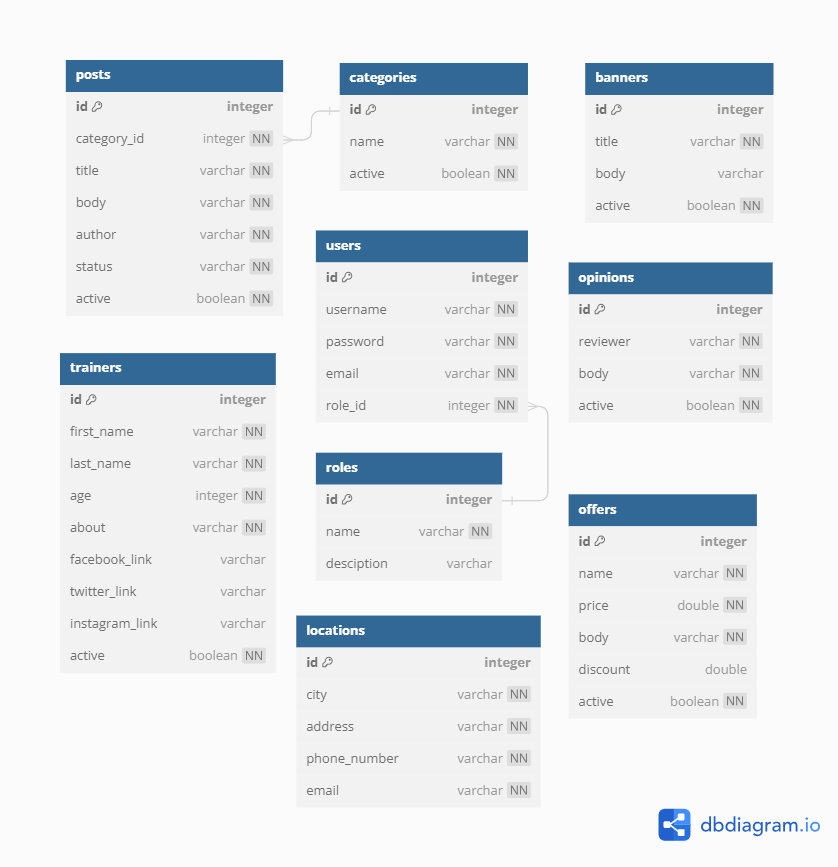
\includegraphics[width=1\textwidth, angle=0]{images/Relational.png}
\newpage
\section{Diagram przypadków użycia}
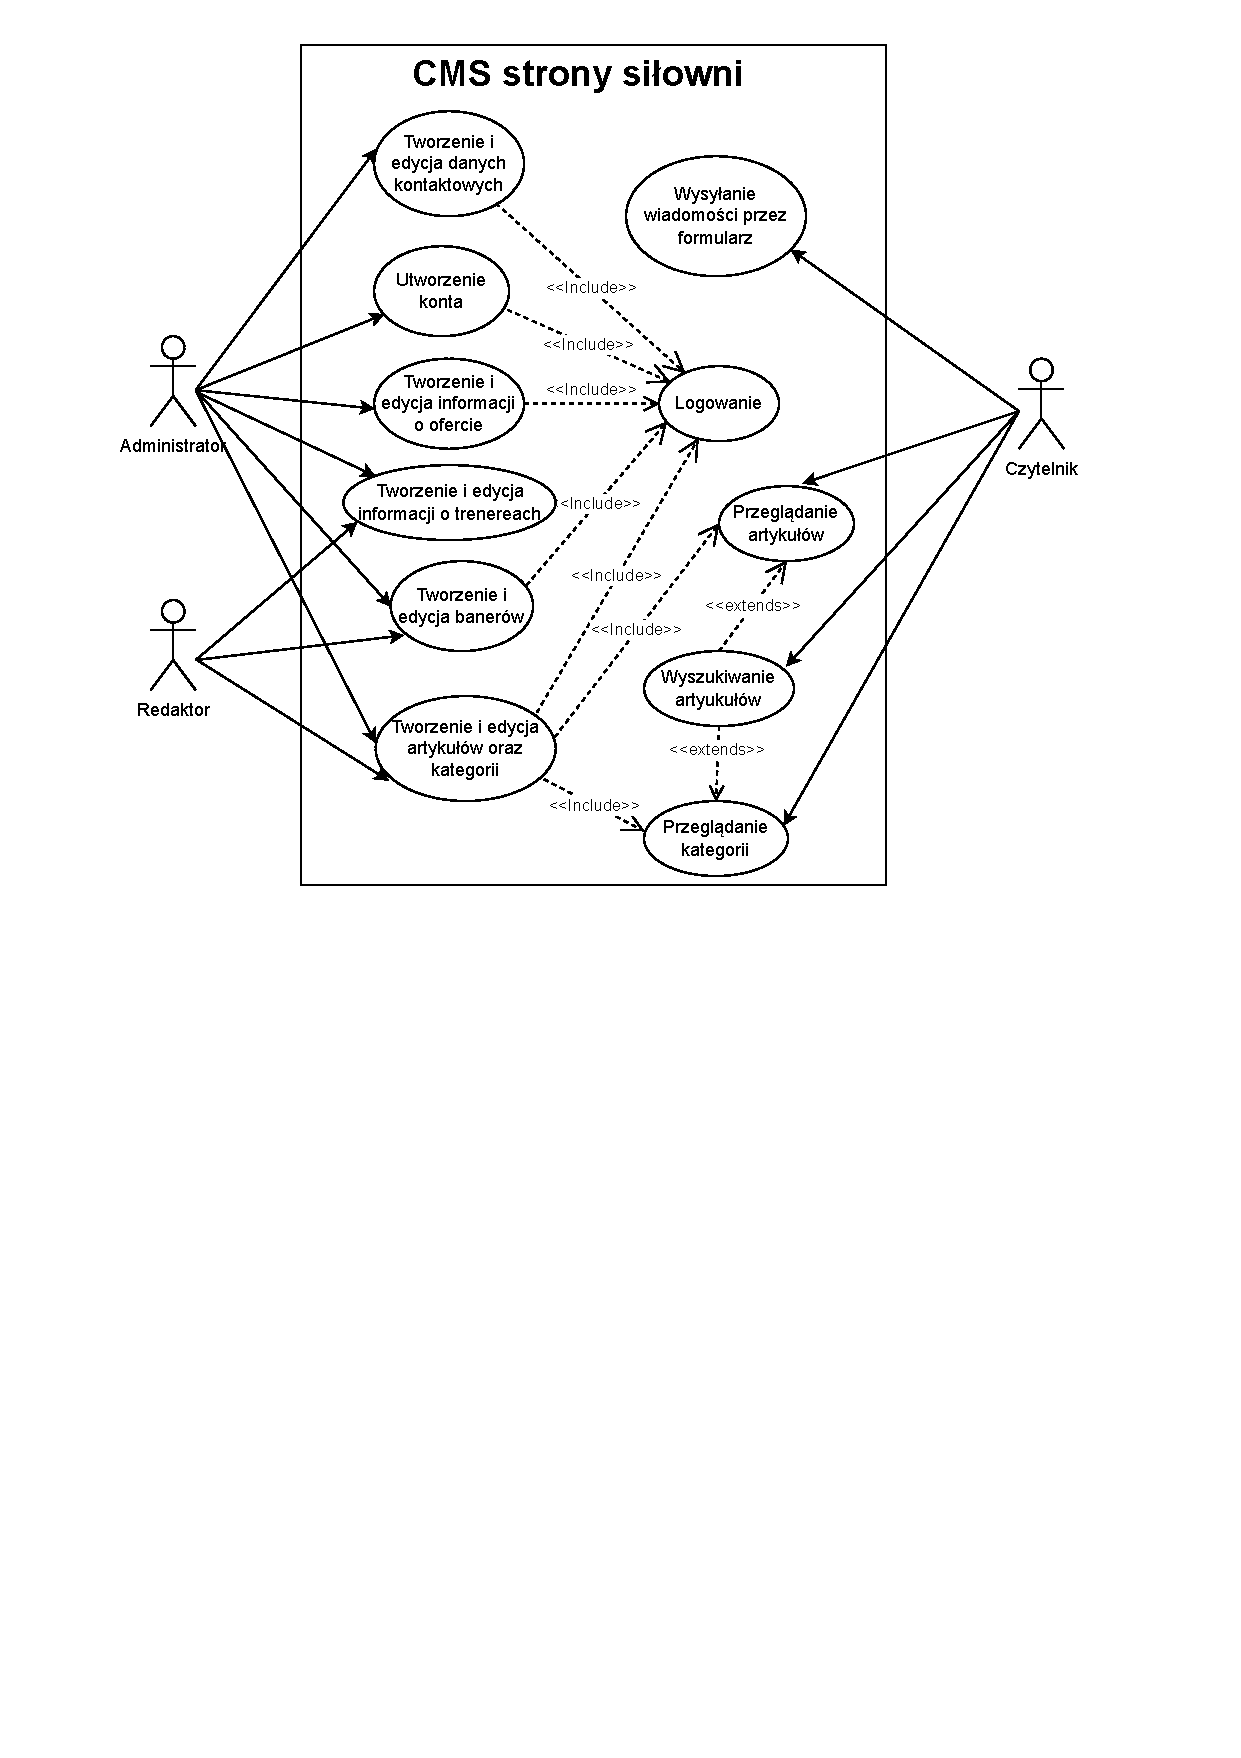
\includegraphics[width=1\textwidth, angle=0]{images/Przypadki_uzycia.pdf}
\newpage
\section{Diagramy klas}
\subsection{Przykładowy diagram backendu}
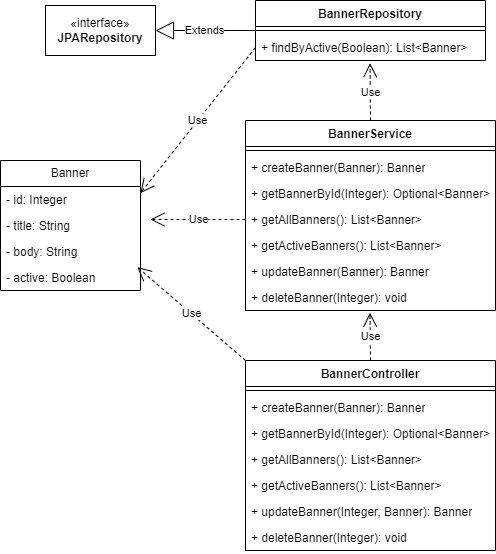
\includegraphics[width=1\textwidth, angle=0]{images/Class_diagram_Java.png}
\subsection{Przykładowy element w API}
\section{Projekty interfejsu graficznego}
\subsection{Panel administratora}
\subsubsection{Lista elementów}
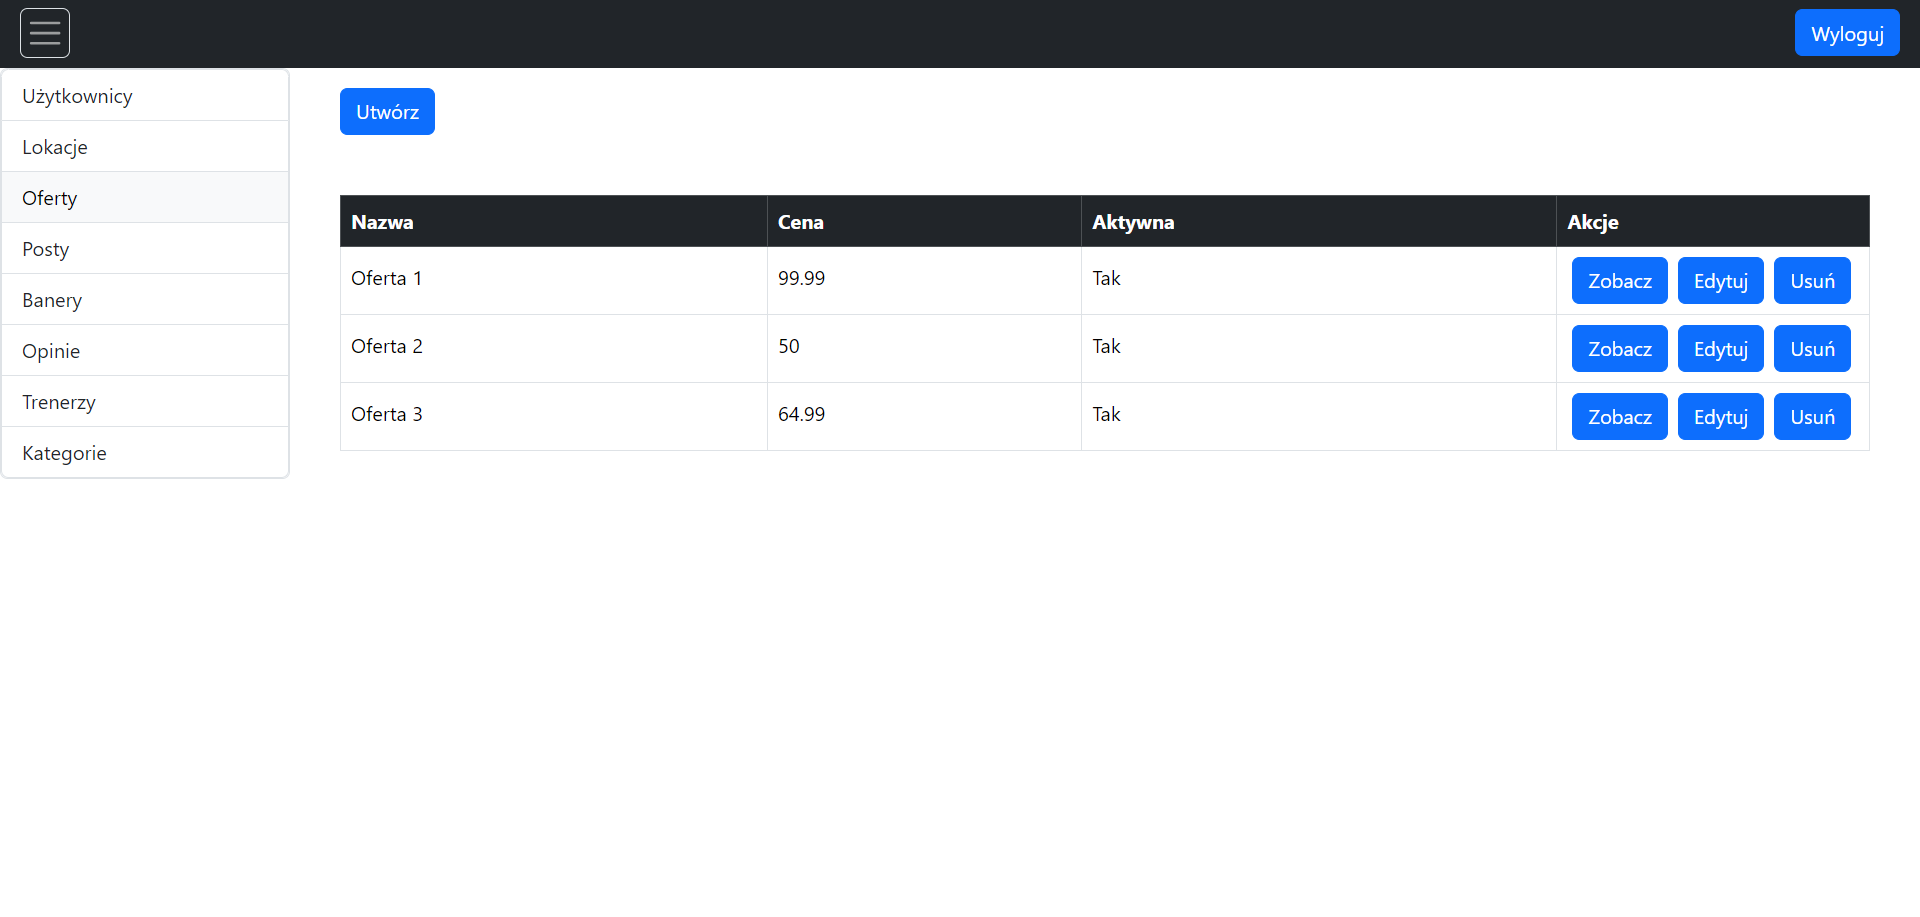
\includegraphics[width=1\textwidth, angle=0]{images/Interface_list.png}
\subsubsection{Ekran logowania}
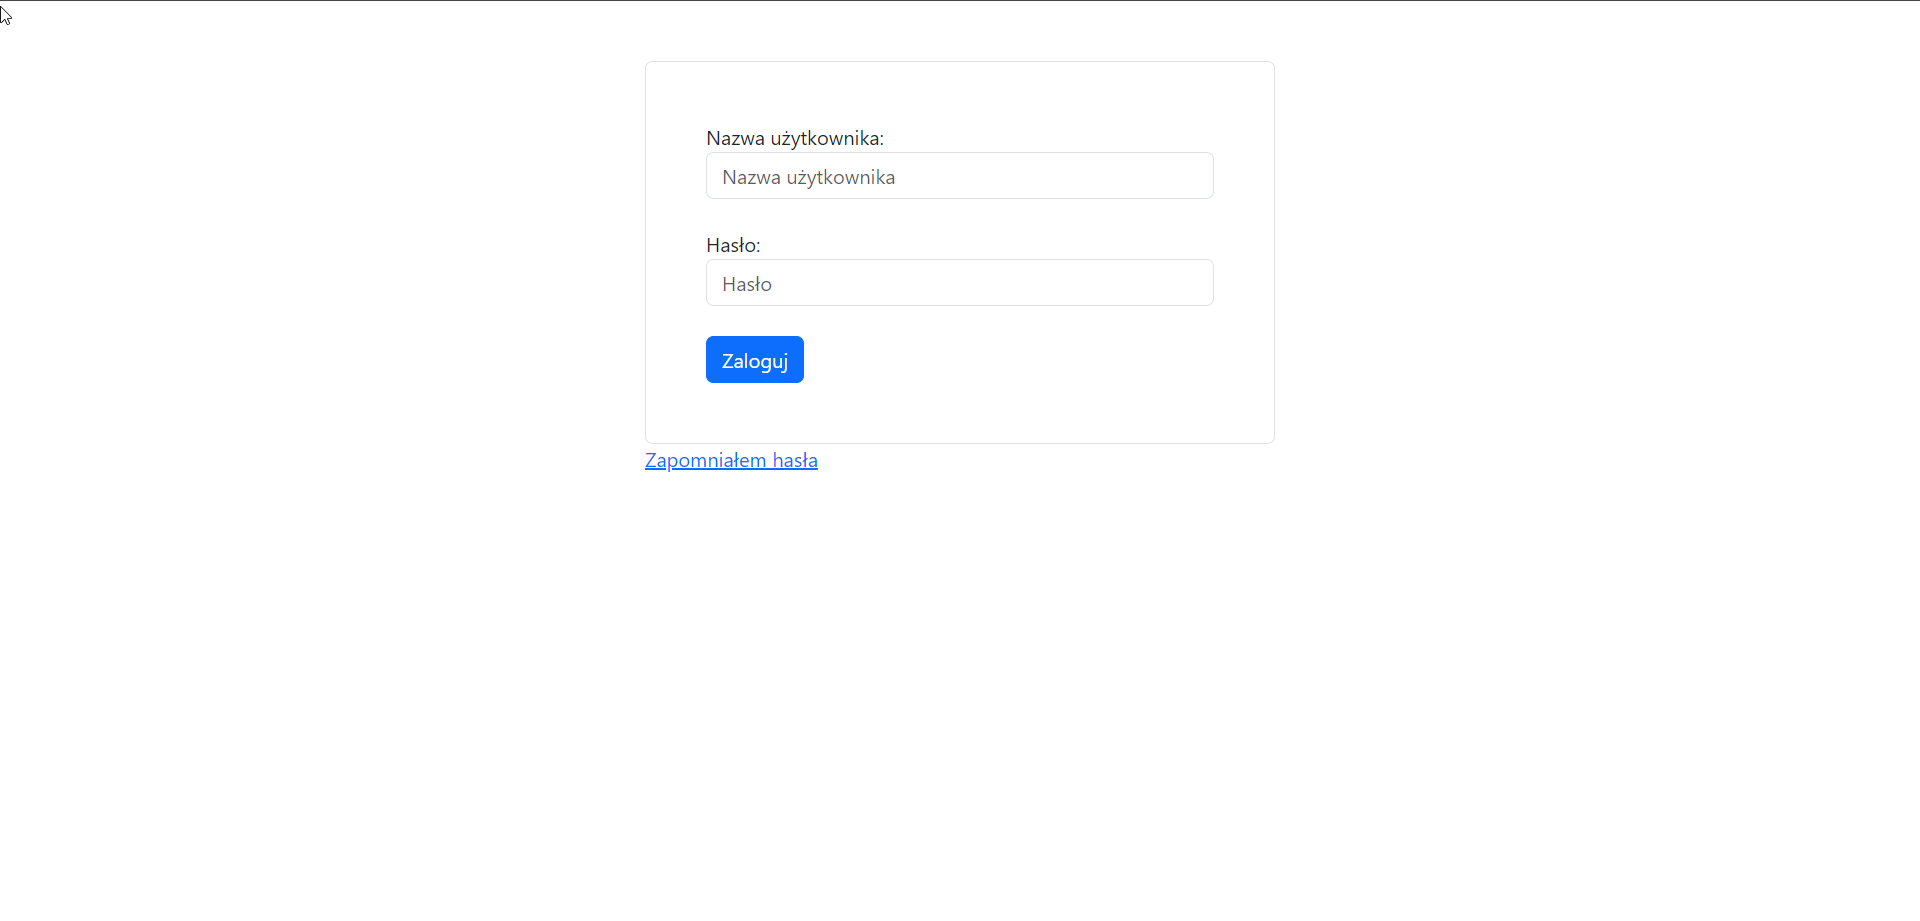
\includegraphics[width=1\textwidth, angle=0]{images/Interface_login.png}
\subsubsection{Ekran widoku elementu}
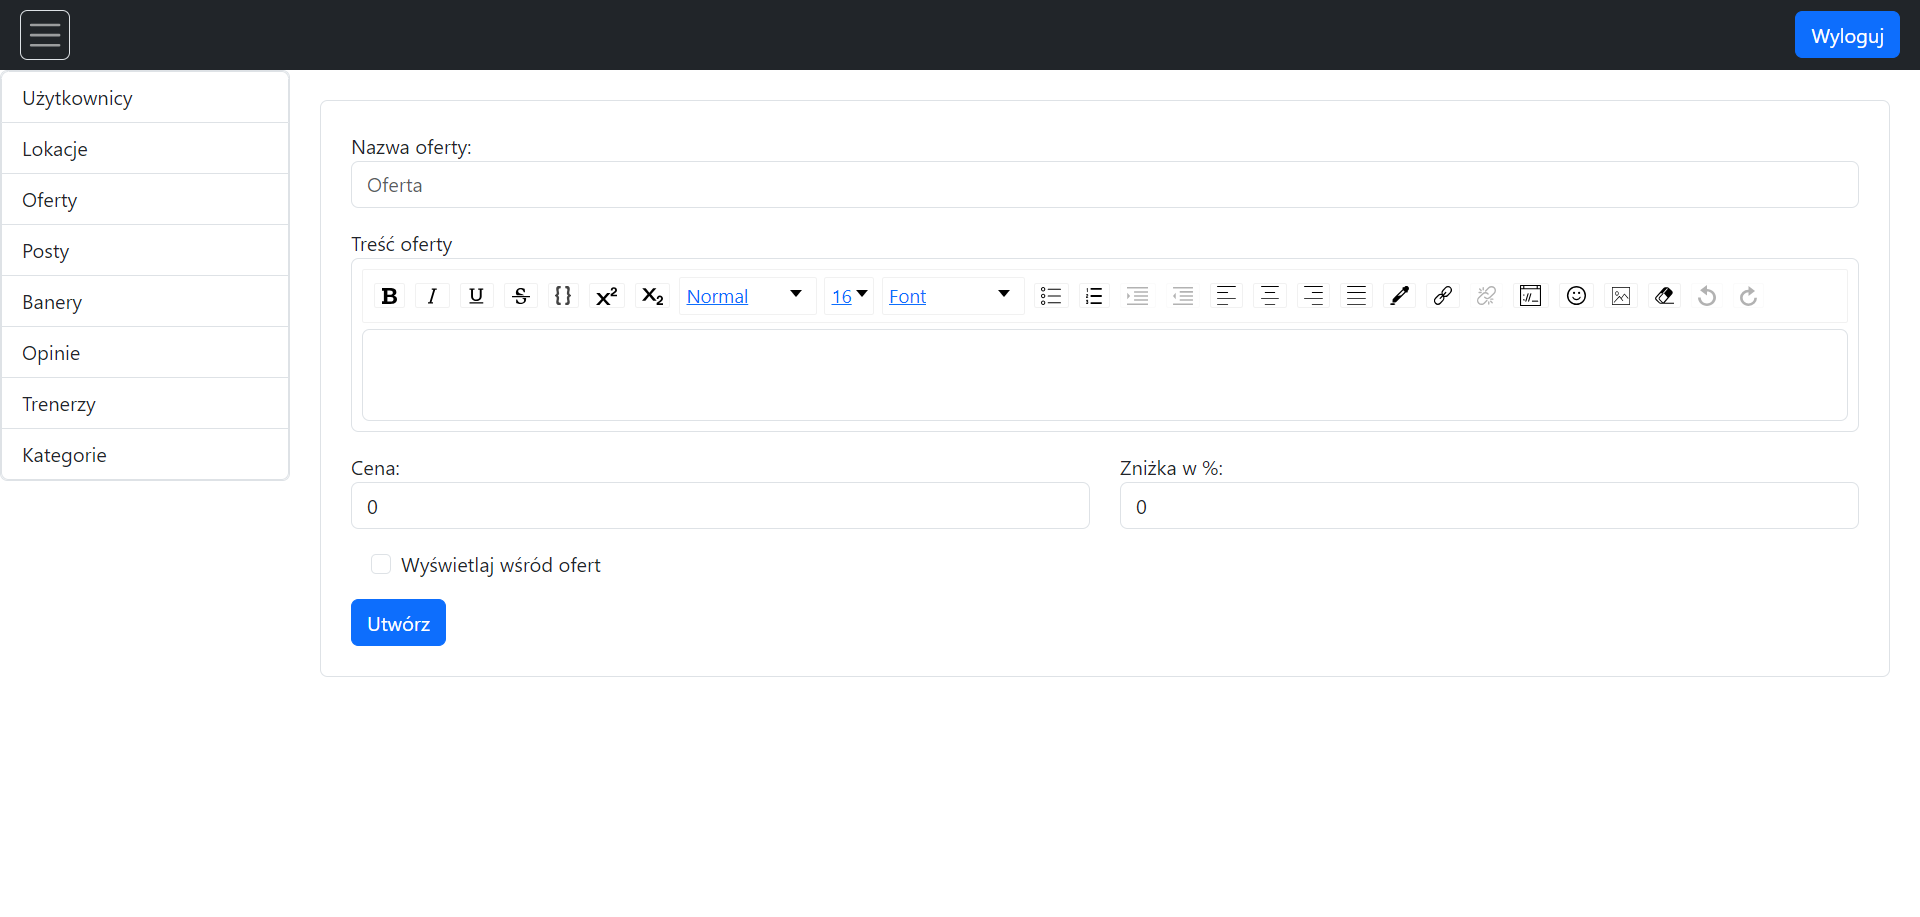
\includegraphics[width=1\textwidth, angle=0]{images/Interface_view.png}

\subsection{Strona główna}
\subsubsection{Homepage - góra}
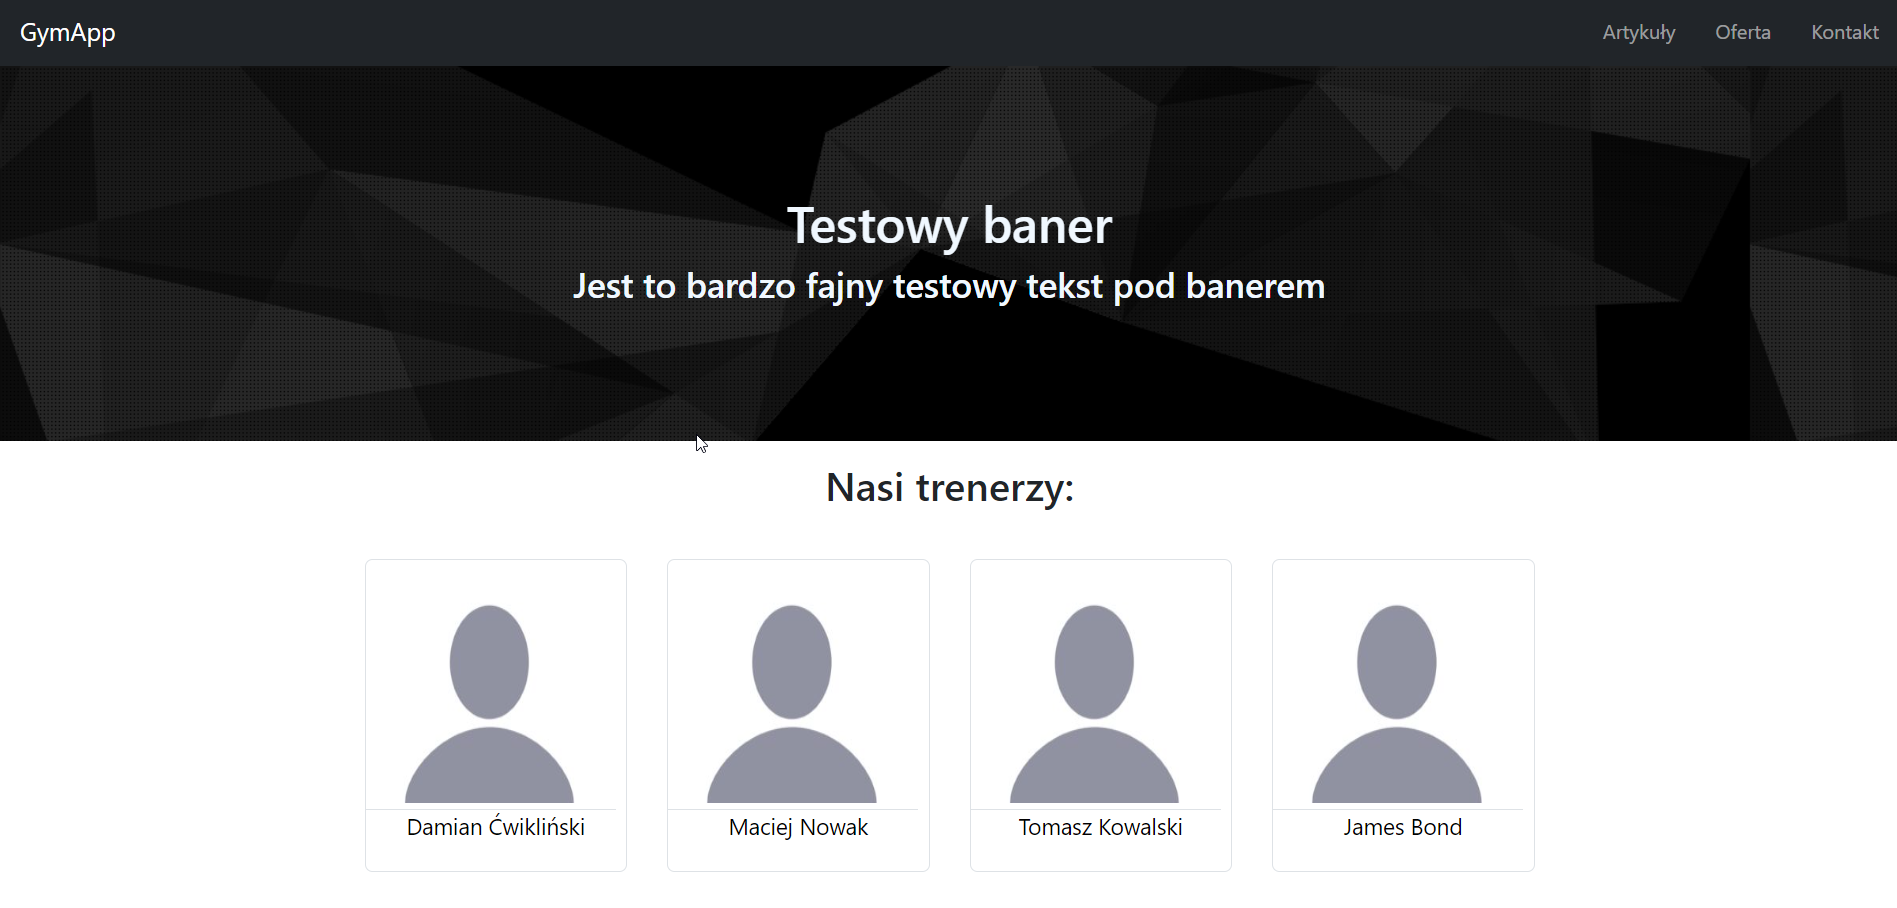
\includegraphics[width=1\textwidth, angle=0]{images/Interface_main1.png}
\subsubsection{Homepage - dół}
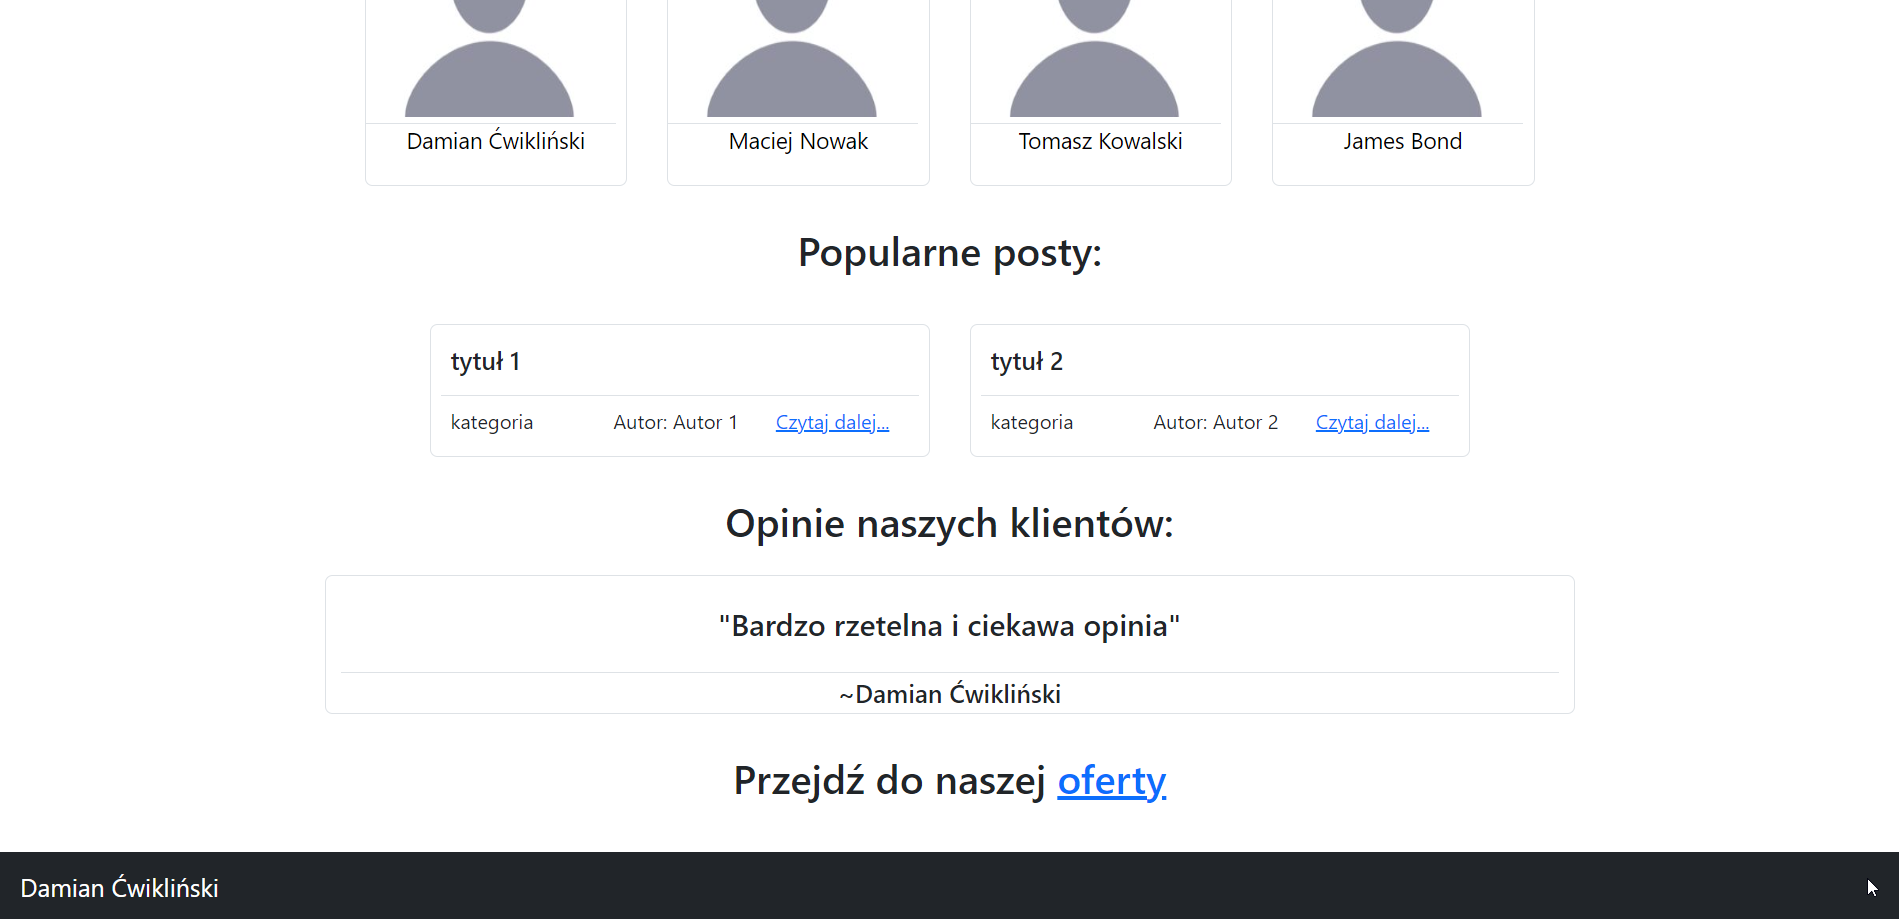
\includegraphics[width=1\textwidth, angle=0]{images/Interface_main2.png}
\subsubsection{Widok ofert}
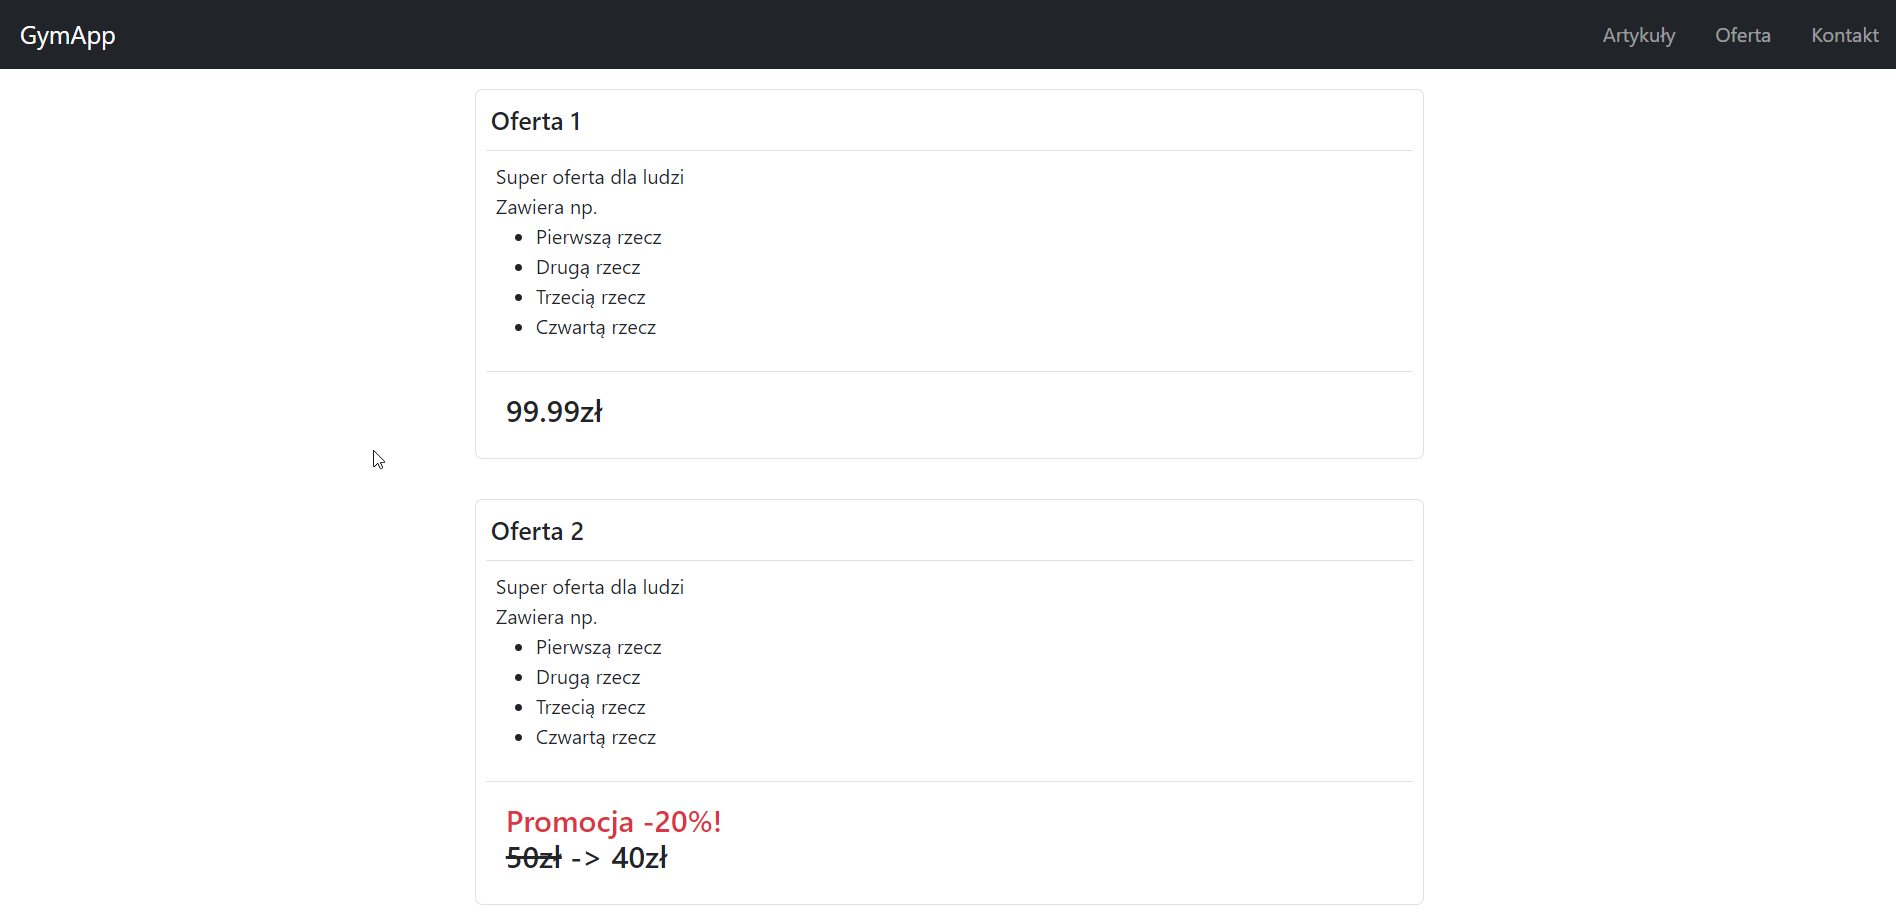
\includegraphics[width=1\textwidth, angle=0]{images/Interface_offers.png}
\subsubsection{Widok posta}
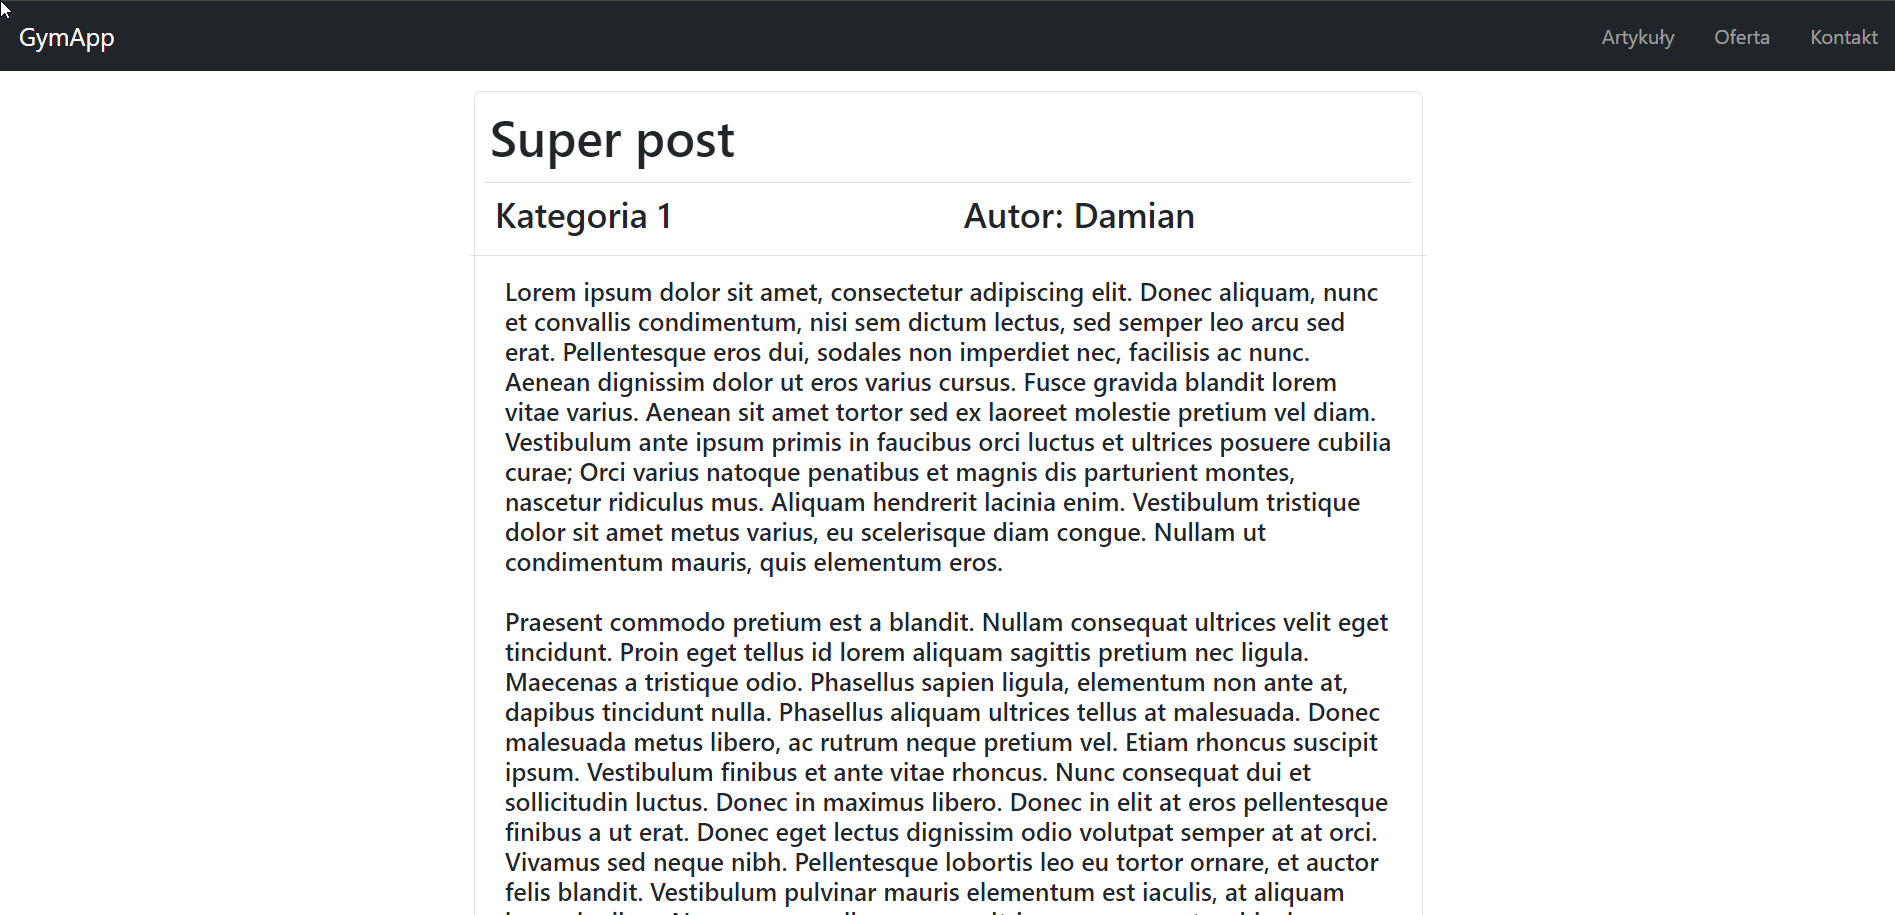
\includegraphics[width=1\textwidth, angle=0]{images/Interface_post.png}
\subsubsection{Dane kontaktowe}
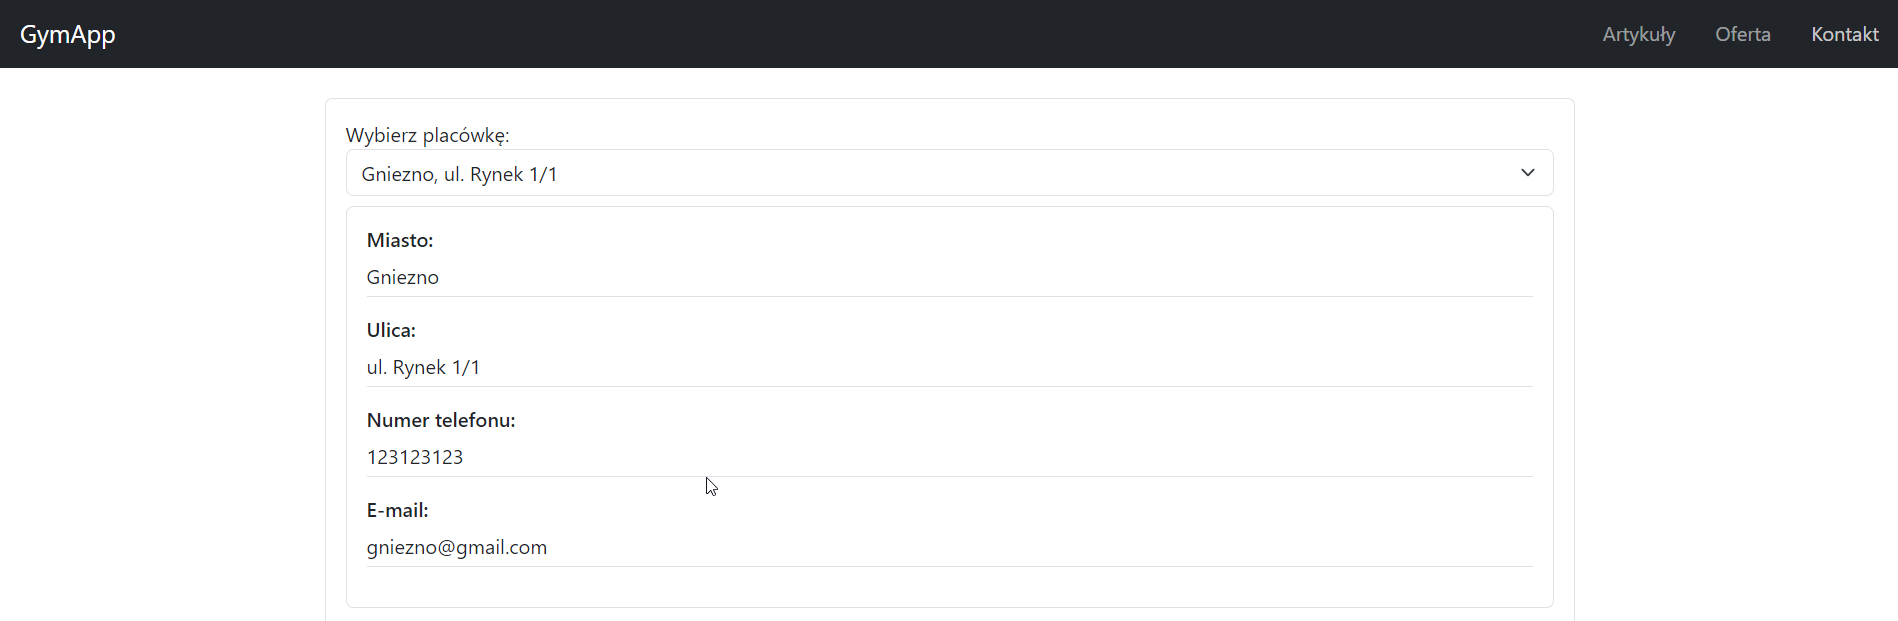
\includegraphics[width=1\textwidth, angle=0]{images/Interface_localization.png}
\subsubsection{Formularz kontaktowy}
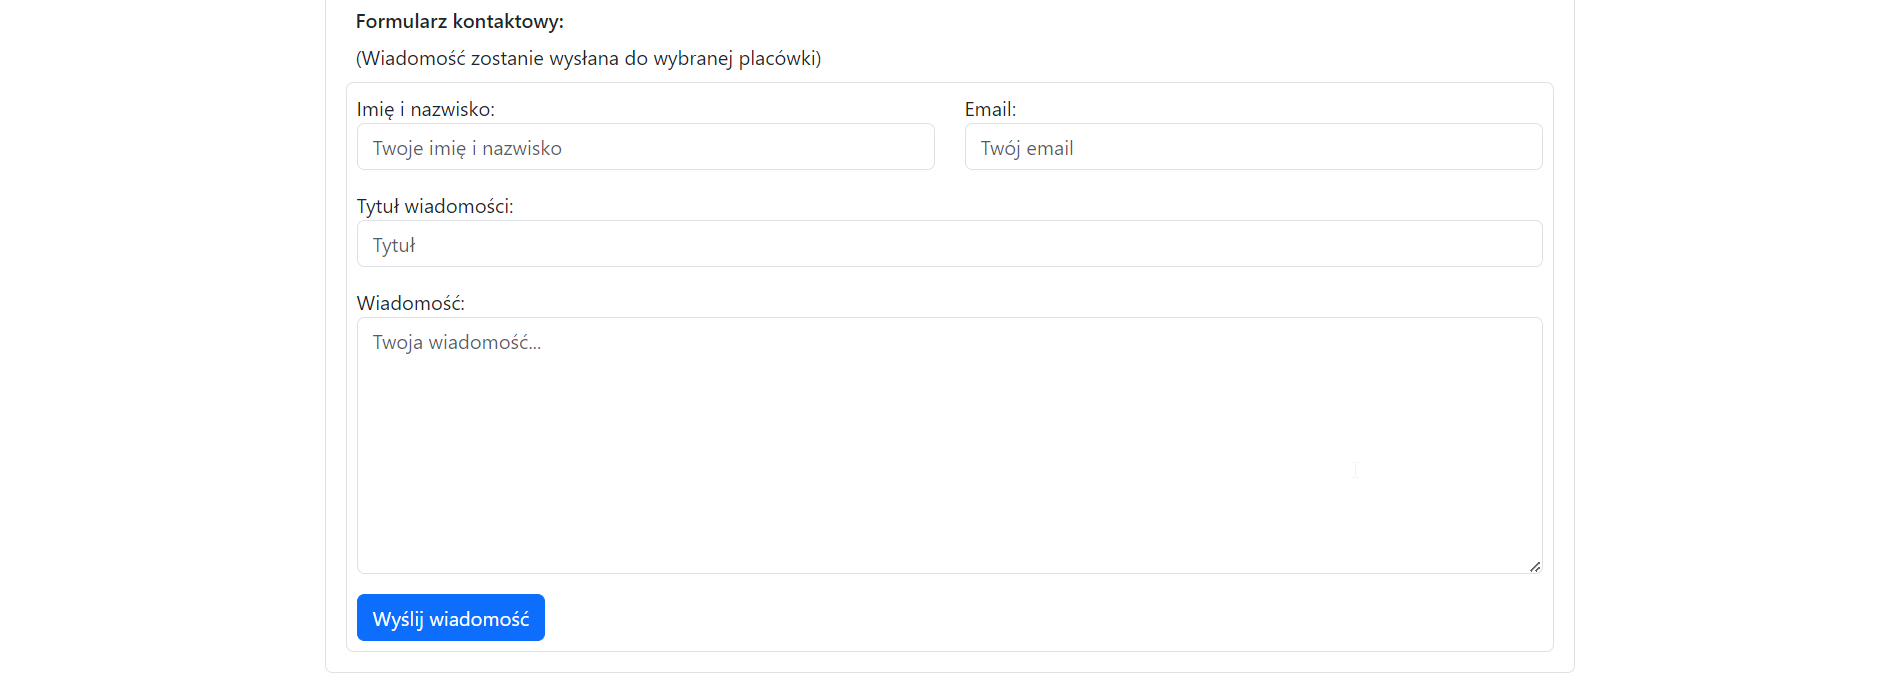
\includegraphics[width=1\textwidth, angle=0]{images/Interface_contact_form.png}
\section{Najważniejsze fragmenty kodu}
Wysyłanie maili
\begin{lstlisting}[language=Java]
@Service
@RequiredArgsConstructor
public class EmailService {
    private final JavaMailSender emailSender;

    public void sendFromContactForm(ContactFormDto message) 
    throws UnsupportedEncodingException, MessagingException{
        sendEmail(message.getSendTo(), message.getSubject(), 
        message.getMessage(), message.getSenderEmail(), 
        message.getSenderName());
    }

    private void sendEmail(String email, String subject, String content, String clientEmail, String clientName)throws MessagingException, UnsupportedEncodingException {
        MimeMessage message = emailSender.createMimeMessage();
        MimeMessageHelper helper = new MimeMessageHelper(message);

        helper.setFrom(clientEmail, clientName);
        helper.setTo(email);
        helper.setSubject("[Formularz] " + subject);
        helper.setText("[" + clientEmail + "]\n" + content);
        
        emailSender.send(message);
    }
}
\end{lstlisting}
\newpage
Konfiguracja zabezpieczeń
\begin{lstlisting}[language=Java]
@Bean
public SecurityFilterChain filterChain(HttpSecurity httpSecurity) 
    throws Exception{
    httpSecurity.csrf(AbstractHttpConfigurer::disable)
        .cors(Customizer.withDefaults())
        .authorizeHttpRequests(auth -> {
            auth.requestMatchers("/api/**").permitAll();
            auth.anyRequest().authenticated();
        })
        .sessionManagement(sessionManagementCustomizer -> {
            sessionManagementCustomizer
        .sessionCreationPolicy(SessionCreationPolicy.STATELESS);
        })
        .authenticationProvider(authenticationProvider)
        .addFilterBefore(jwtAuthenticationFilter, 
        UsernamePasswordAuthenticationFilter.class)
        .httpBasic(Customizer.withDefaults());
return httpSecurity.build();
}
\end{lstlisting}

Tworzenie tokena JWT
\begin{lstlisting}[language=Java]
Tworzenie tokena JWT
private String buildToken(
    Map<String, Object> extraClaims,
    UserDetails userDetails,
    long expiration
) {
    return Jwts
        .builder()
        .setClaims(extraClaims)
        .setSubject(userDetails.getUsername())
        .setIssuedAt(new Date(System.currentTimeMillis()))
        .setExpiration(new Date(System.currentTimeMillis() + expiration))
        .signWith(getSignInKey(), SignatureAlgorithm.HS256)
        .compact();
    }
\end{lstlisting}
\newpage
Pobieranie elementu z API
\begin{lstlisting}
export const getOneObject = async (id: string | undefined, 
endpoint: string, setData: (data: SetStateAction<any>) => void) => {
    try {
        await axios.get(`http://localhost:8080/api/${endpoint}/${id}`, 
        config).then(response => {
            console.log(response)
            if (response.status === 200) {
                setData(response.data)
            }
            else {
                console.log("Could not get data");
            }
        })
    } catch (error) {
        console.error('Error during fetching:', error);
    }
}
\end{lstlisting}
Funkcja logowania do aplikacji
\begin{lstlisting}
try {
      const response = await axios.post('http://localhost:8080/api/auth/login', loginData);

      if (response.status === 200) {
        sessionStorage.setItem("token", response.data.token);
        sessionStorage.setItem("role", response.data.roleName);
        navigate("/manage");
      } else {
        console.error('Login failed');
      }
    } catch (error) {
      console.error('Error during login:', error);
    }
\end{lstlisting}
\newpage
Tworzenie listy z elementami
\begin{lstlisting}
const renderCrudButtons = (id: number): ReactNode => {
    return(
        <td className='btns-crud'>
            <Link className='mx-1' to={id.toString()}>
                <button className='btn btn-primary'>Zobacz</button>
            </Link>
            <Link className='mx-1' to={id + "/edit"}>
                <button className='btn btn-primary'>Edytuj</button>
            </Link>
            <Link className='mx-1' to={""}>
                <button className='btn btn-primary' onClick={() => handleDelete(id)}>Usun</button>
            </Link>
        </td>)}

const renderHeaders = (headers: Array<string>): ReactNode => {
    return headers.map(header => <th key={header}>{header}</th>)}
    

function renderListItems(items: Array<ListItem>) {
    if (items.length != 0){
        return items.map(item => <tr key={`${item.id}`}>{item.content.map(cell => <td key={`${item.id}${cell}`}>{cell}</td>)}{renderCrudButtons(item.id)}</tr>)
    }
    return <tr key='1'>Brak danych do wyswietlenia</tr>
}
    
return (
    <div className='container p-3'>
        <Link to="create">
            <button className='btn btn-primary'>Utworz</button>
        </Link>
        <table className='table table-bordered border mt-5'>
            <thead className='table-dark'>
                <tr key="0">
                    {renderHeaders([...headers, "Akcje"])}
                </tr>
            </thead>
            <tbody>
                {renderListItems(items)}
            </tbody>
        </table>
    </div>)
\end{lstlisting}
\begin{lstlisting}
\end{lstlisting}
\section{Analiza bezpieczeństwa}
Strona nie przechowuje żadnych danych wrażliwych, co oznacza, że bezpieczeństwo choć ważne, nie jest priorytetem. Użytkownikami systemu z założenia są osoby zaufane.
\\

Do zabezpieczenia elementów po stronie backendu wykorzystano bibliotekę spring security oraz tokeny JWT. Tokeny nie pozwalają na dostęp do danych nieupoważnionym osobom nawet gdyby odnalazły endpointy, bądź dostały się nieupoważnienie do chronionych części strony.
\\

Po stronie frontendu zablokowano pewne możliwości osobom niezalogowanym lub z za niskimi uprawnieniami. Zakładki dostępne dla admina są chowane, gdy zalogowany jest zwykły użytkownik, nieautoryzowana próba wejścia do chronionych części aplikacji kończy się wyrzuceniem osoby na stronę logowania.
\\

Elementy tworzone edytorem tekstu tak jak treść posta, konwertowana jest na format JSON co powinno zabezpieczyć przed niechcianymi egzekucjami kodu.
\section{Podsumowanie}
\subsection{Cele zrealizowane}
\begin{itemize}
\item Główna strona z banerami, ofertami, postami, informacjami kontaktowymi
\item Formularz kontaktowy wysyłający maile na adresy placówek
\item Panel admina pozwalający na edycję głównej strony
\item Logowanie do panelu admina oraz zabezpieczenie aplikacji przy pomocy tokenów JWT
\item Podział na konta użytkowników i administratorów
\item Edycja, dodawanie i usuwanie
\begin{itemize}
\item banerów
\item użytkowników
\item postów
\item kategorii
\item oferty
\item informacji kontaktowych
\item trenerów
\item opinii klientów
\end{itemize}
\end{itemize}
\subsection{Cele niezrealizowane}
\begin{itemize}
\item Dodawanie obrazów przez użytkownika
\item Resetowanie hasła
\item Brak testów jednostkowych
\end{itemize}
\subsection{Napotkane problemy}
\begin{itemize}
\item Słaba znajomość wybranych technologii
\item Problemy z konfiguracją usługi SMTP
\item Decyzja o zrobieniu wszystkiego od zera z perspektywy czasu była złą decyzją

\end{itemize}
\subsection{Perspektywa rozwoju}
\begin{itemize}
\item Zmiana zdjęć trenerów i różne obrazy dla banerów
\item Dodanie dodatkowych sekcji na stronie głównej
\item Dodanie kolejnych zakładek w górnym pasku
\item Opcje wyszukiwania postów
\item Formularz kontaktowy dla trenerów
\item możliwość zmieniania kolejności elementów strony 
\end{itemize}
\end{document}
